\subsection{Reproducing the Grokking Curve}
\label{sec:subtask1}

In this task, we investigate the grokking phenomenon in modular addition with the transformer model.
Specifically, we use a decoder-only transformer with $2$ layers, width $d_{\mathrm{model}} = 128$, $4$ attention heads and dropout $0.1$.
We use the AdamW optimizer with $\beta_1 = 0.9, \beta_2 = 0.98$, learning rate $10^{-3}$, weight decay $0.1$, and linear learning rate warmup over the first $10$ updates.
For $p = 97$ and $\alpha = 0.5$, we randomly separate an $\alpha$ fraction from all $p^2$ equations in $\ZZ_p$ as the training set; the rest serves as the validation set.
The model is trained with minibatch size $512$ for $10^5$ steps.

The accuracy and loss throughout the training process are plotted in \cref{fig:acc_and_loss_transformer}.

\begin{figure}[!ht]
    \centering
    \begin{subfigure}{0.45\textwidth}
        \centering
        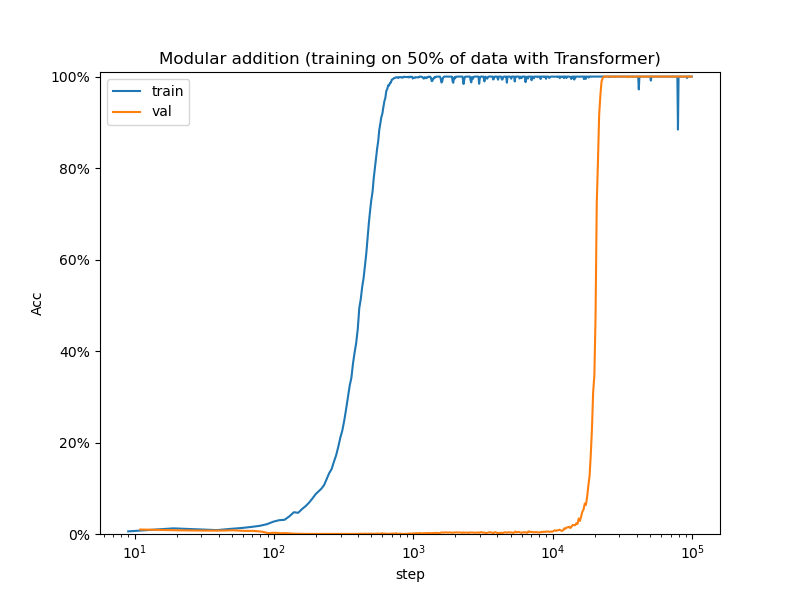
\includegraphics[width=\linewidth]{fig/grokking_curves/addition_50_Transformer_step.png}
        \caption{Training and validation accuracy}
        \label{fig:grokking_curve_transformer}
    \end{subfigure}
    %\hfill
    \begin{subfigure}{0.45\textwidth}
        \centering
        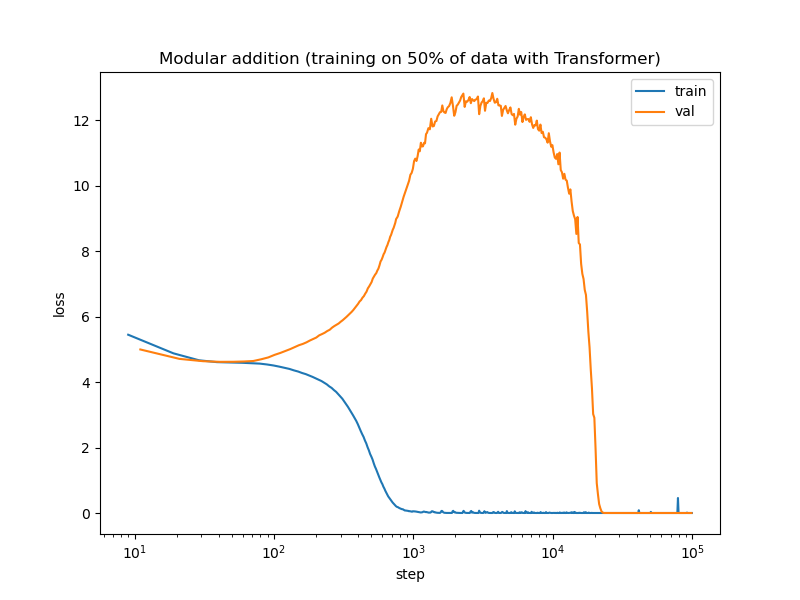
\includegraphics[width=\linewidth]{fig/loss_curves/addition_50_Transformer_step.png}
        \caption{Training and validation loss}
        \label{fig:loss_curve_transformer}
    \end{subfigure}

    \caption{The grokking curves of transformer model}
    \label{fig:acc_and_loss_transformer}
\end{figure}

As is shown in \cref{fig:grokking_curve_transformer}, the model overfits the training data within $10^3$ updating steps.
Nevertheless, generalization does not happen until after $10^4$ steps.
\cref{fig:loss_curve_transformer} further illustrates that the decrease of loss is consistent with the increase of accuracy, both for training and validation phases.
Interestingly, while the training loss decreases monotonically, an increase of the validation loss is observed before it begins to converge.

We further study the effect of the training data fraction $\alpha$. 
For each $\alpha$ we sample, we train the model on a random $\alpha$ fraction of all $p^2$ equations for at most $10^5$ steps, and determine the minimum number of steps required to achieve validation accuracy $\geq 99\%$.
The results are plotted in \cref{fig:transformer_alpha}.
As a comparison, we plot the accuracy curves for $\alpha = 80\%$ and $\alpha = 33\%$ in \cref{fig:grokking_alpha_80,fig:grokking_alpha_33}, respectively.

\begin{figure}[!ht]
    \centering
    \begin{subfigure}[t]{0.3\textwidth}
        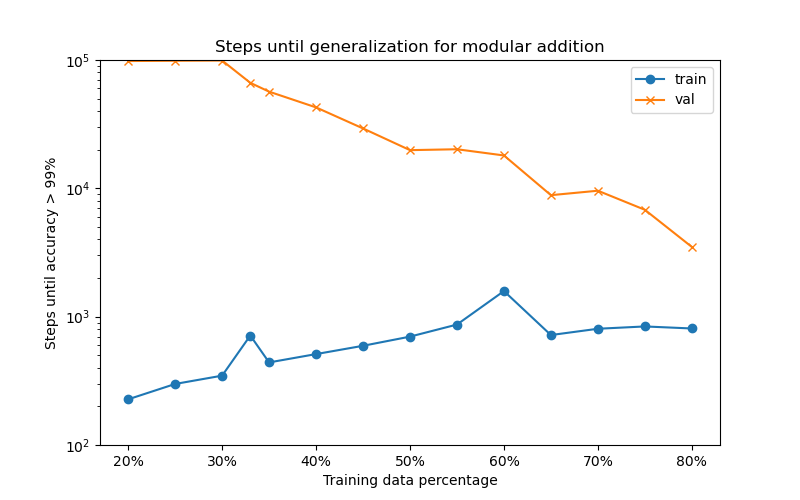
\includegraphics[width=\linewidth]{fig/Transformer_alpha/Transformer_alpha.png}
        \caption{Minimal number of training steps required to achieve validation accuracy $\geq 99\%$}
        \label{fig:transformer_alpha}
    \end{subfigure}
    \hfill %
    \begin{subfigure}[t]{0.3\textwidth}
        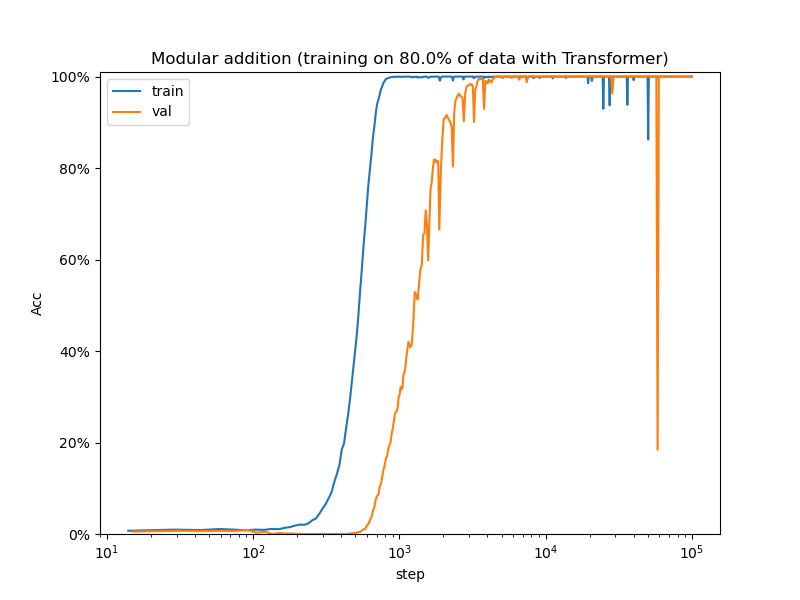
\includegraphics[width=\linewidth]{fig/grokking_curves/addition_80.0_Transformer_step.png}
        \caption{The accuracy curve for $\alpha = 80\%$}
        \label{fig:grokking_alpha_80}
    \end{subfigure}
    \hfill %
    \begin{subfigure}[t]{0.3\textwidth}
        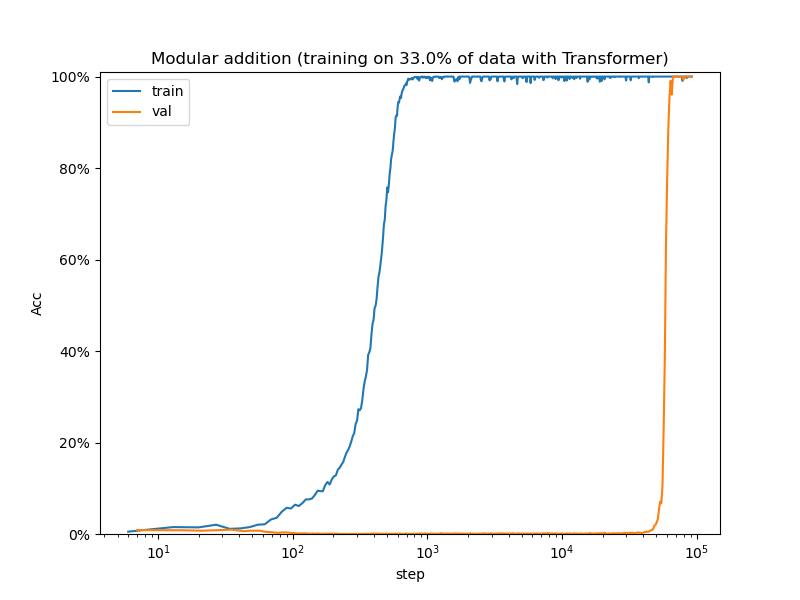
\includegraphics[width=\linewidth]{fig/grokking_curves/addition_33.0_Transformer_step.png}
        \caption{The accuracy curve for $\alpha = 33\%$}
        \label{fig:grokking_alpha_33}
    \end{subfigure}

    \caption{Effect of the training data fraction $\alpha$}
    \label{fig:effect_of_alpha}
\end{figure}

When $\alpha = 80\%$, the model generalizes in $10^4$ steps.
As $\alpha$ decreases, it becomes easier for the model to overfit the training data, while the number of steps required for generalization increases rapidly.
When $\alpha \leq 30\%$, the model would not generalize in $10^5$ steps.